\appendix

\section{Supplementary Figures and Tables}
\label{sec:appendix:tables}

\input{sections/_inbody_deployer}
% In-body frontier table (plus-page camera-ready). Locked numbers only.
%   Anthropic 4.x pooled C0  0/2,592  <=0.14%
%   OpenAI gpt-4.x/4o (5)    0/2,117  <=0.18%
%   gpt-5 generation (4)     0/1,311  <=0.28%  (CONFIRMATORY, out of headline pool)
%   Qwen3 peak (14B) 6/366=1.64%; Qwen2.5-7B 28/459=6.10%; Llama-3.1-8B 5/400=1.25%
\begin{table}[t]
\caption{Tool-fabrication rate (TFR) on the target-removed distractor
probe ($\mathrm{C}_0$): the commercial frontier vs.\ the open-weight band.
Cells are events\,/\,parsed calls; UB is the two-sided Clopper--Pearson
$95\%$ upper bound. This is an \emph{open-vs-closed} split, not a verified
model property: every commercial tier is reached through its vendor's
structured function-calling API (which can refuse or drop a malformed
call), whereas every open-weight model is a self-hosted $4$-bit MLX build
whose calls we recover by text-parsing the generated stream. The two reach
paths cannot be separated, so we report the contrast as a serving-and-model
bundle and draw no scaling law or cross-vendor capability ranking from it.
The gpt-5 generation is a confirmatory extension, kept out of the locked
$0/2{,}117$ OpenAI headline pool.}
\label{tab:frontier}
\centering
\small
\setlength{\tabcolsep}{3pt}
\begin{tabular}{llr}
\toprule
Tier & Events\,/\,$N$ & TFR (UB) \\
\midrule
\multicolumn{3}{l}{\emph{Commercial (closed, API-served)}} \\
Anthropic 4.x (5 ver., pooled) & $0/2{,}592$ & $0\%$ {\scriptsize($\leq\!0.14\%$)} \\
OpenAI gpt-4.1/4o (5 tiers)    & $0/2{,}117$ & $0\%$ {\scriptsize($\leq\!0.18\%$)} \\
OpenAI gpt-5 gen.\ (4)         & $0/1{,}311$ & $0\%$ {\scriptsize($\leq\!0.28\%$)} \\
\midrule
\multicolumn{3}{l}{\emph{Open-weight (4-bit MLX, text-parsed)}} \\
Qwen3 (peak, $14$B)            & $6/366$  & $1.64\%$ \\
Qwen2.5-7B                     & $28/459$ & $6.10\%$ \\
Llama-3.1-8B                   & $5/400$  & $1.25\%$ \\
\bottomrule
\end{tabular}
\end{table}


\begin{figure}[tb]
\centering
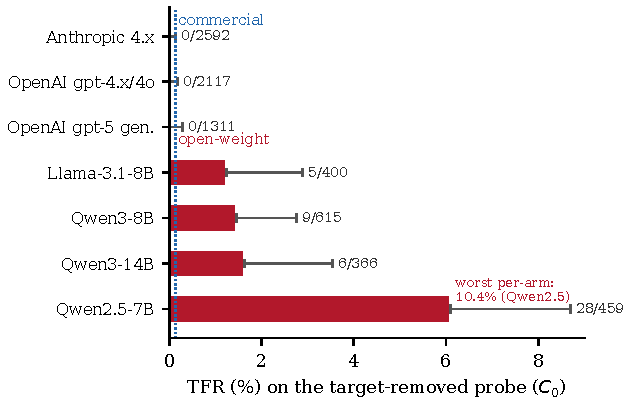
\includegraphics[width=\linewidth]{figures/figA_commercial_open}
\caption{Commercial versus open-weight TFR on the target-removed
$\mathrm{C}_0$ probe. Five Anthropic 4.x versions ($0/2{,}592$), the
OpenAI gpt-4.x/4o tiers ($0/2{,}117$), and the gpt-5 generation
($0/1{,}311$) log zero fabrications; open-weight lineages fabricate at
$1.25$ to $6.10\%$, with the worst per-arm cell at $10.4\%$ (Qwen2.5,
synonym distractor). Error bars are Clopper--Pearson $95\%$ upper
bounds.}
\label{fig:commercial-open}
\end{figure}

\begin{figure}[tb]
\centering
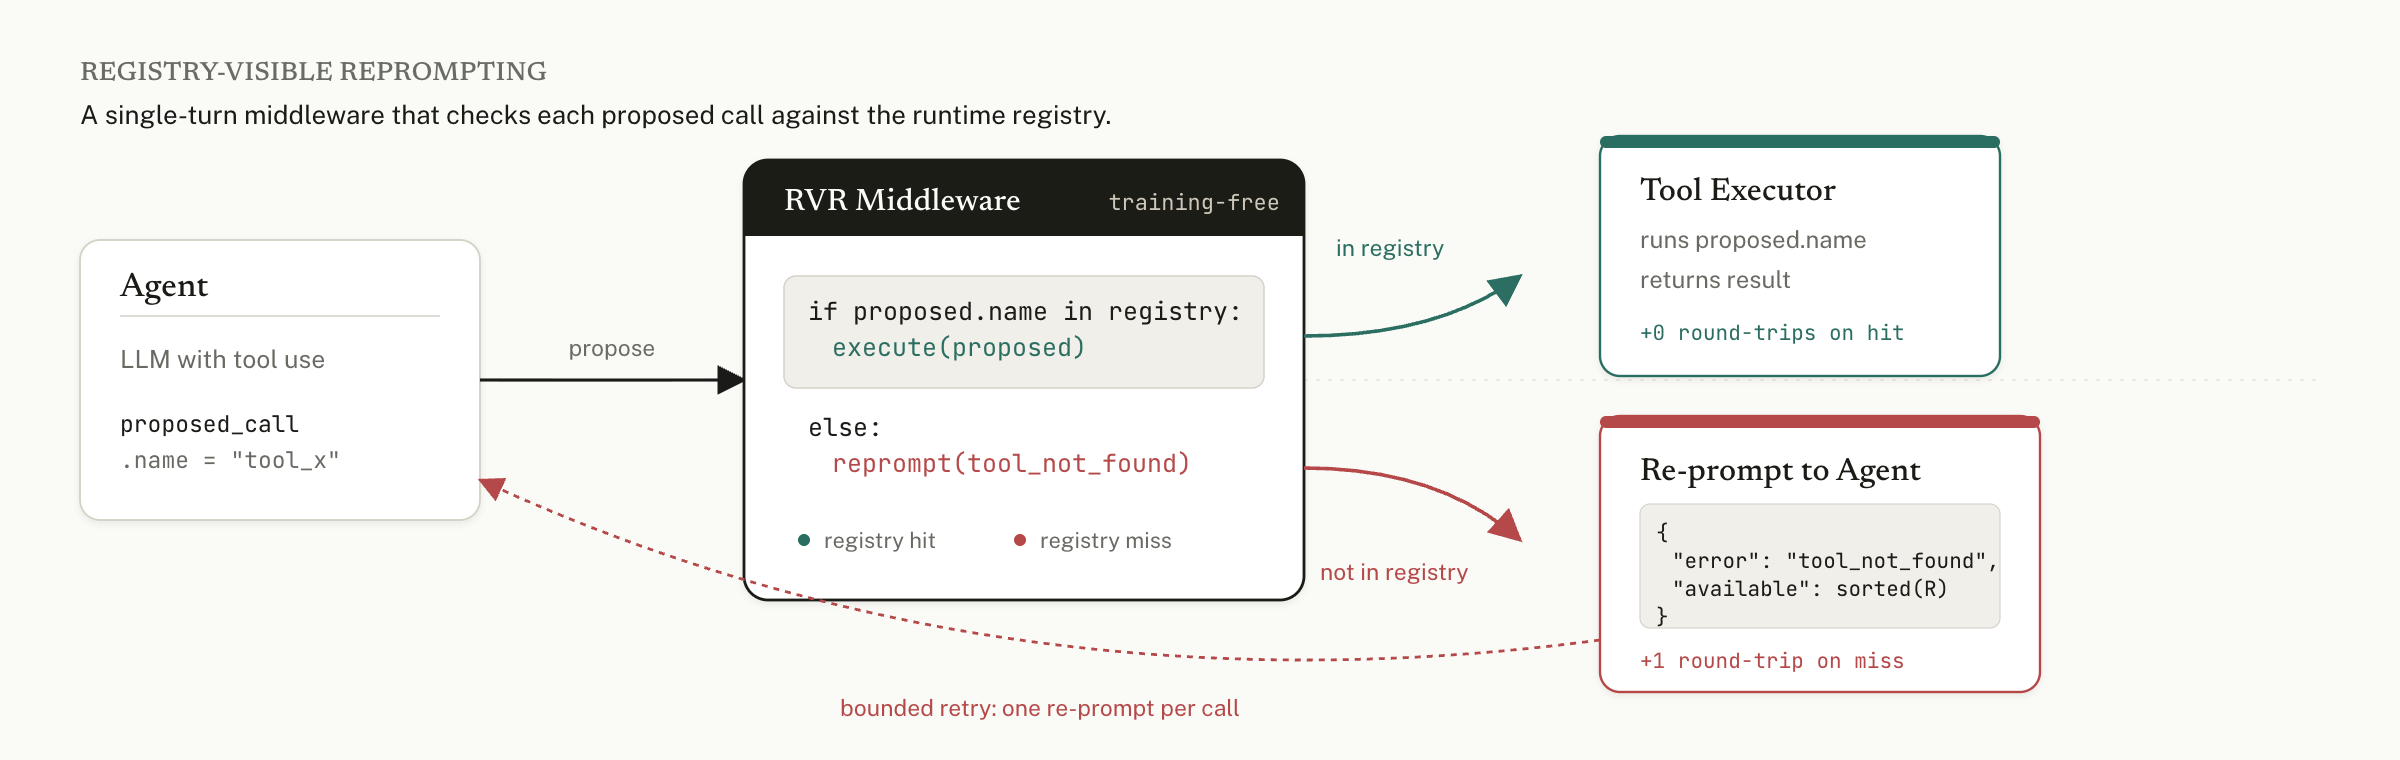
\includegraphics[width=\linewidth]{figures/fig3_rvr_architecture}
\caption{RVR middleware. An $O(1)$ membership check runs in-process
on each proposed call. Hits execute. Misses trigger one re-prompt
with a structured \texttt{tool\_not\_found} envelope (and the sorted
registry under $\mathrm{C}_1$). The no-violation path adds zero
provider round-trips; the violation path adds one, bounded to a
single retry.}
\label{fig:rvr-arch}
\end{figure}

\begin{figure}[tb]
\centering
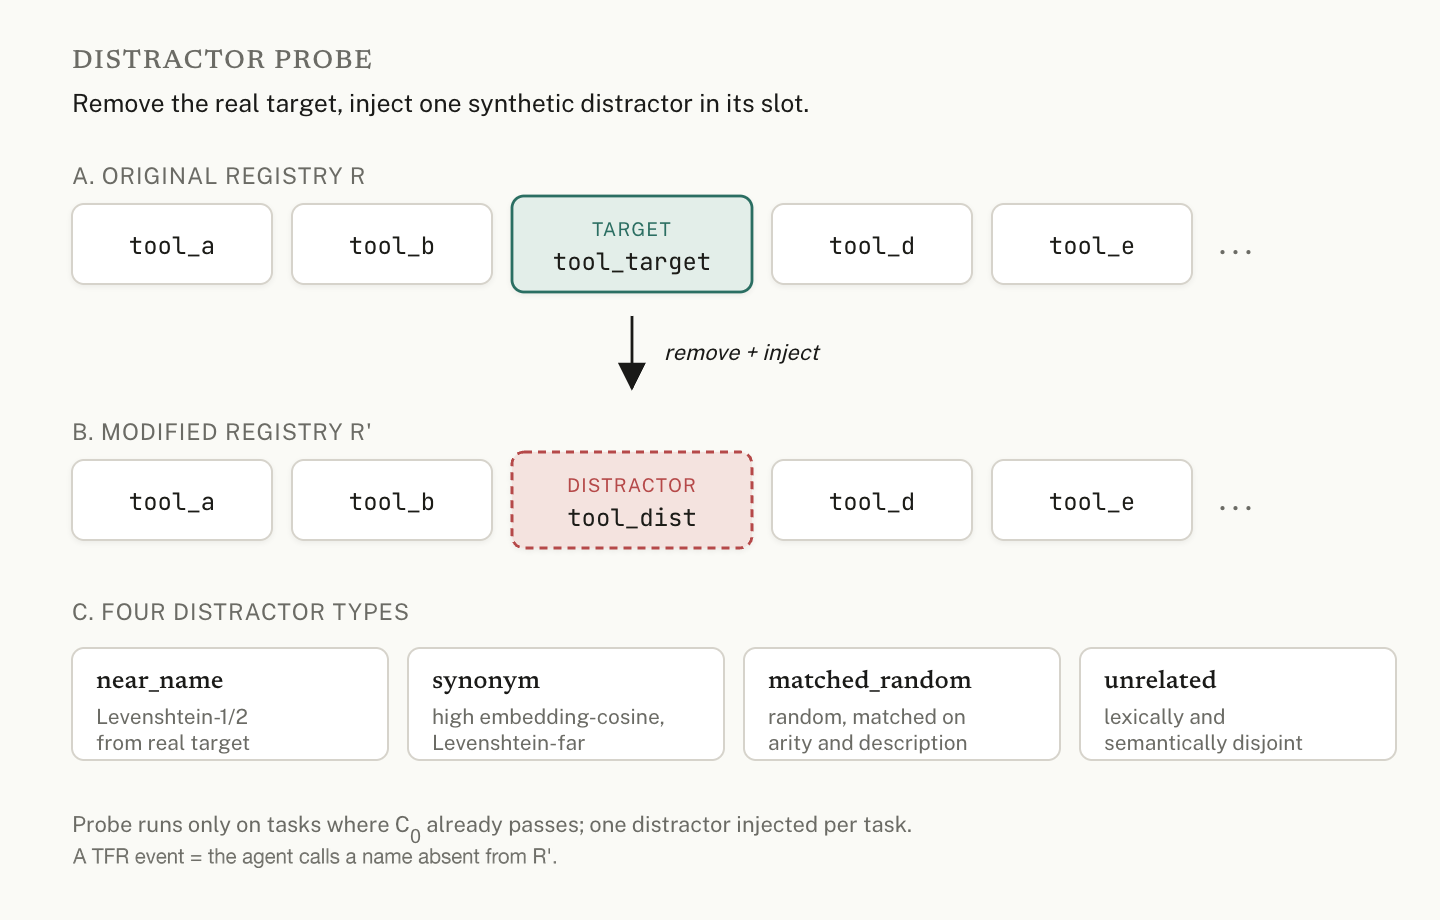
\includegraphics[width=0.82\linewidth]{figures/fig4_distractor_probe}
\caption{The distractor probe. Starting from a registry where the
opaque baseline already passes, the real target tool is removed and
one synthetic distractor is injected in its slot. The four arms vary
the similarity profile of the distractor.}
\label{fig:probe}
\end{figure}

\begin{figure}[tb]
\centering
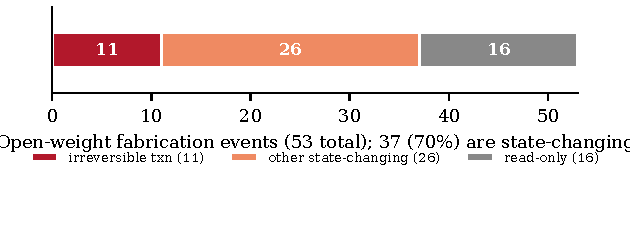
\includegraphics[width=\linewidth]{figures/figB_severity}
\caption{What gets fabricated. Of the $53$ open-weight $\mathrm{C}_0$
fabrication events, $37$ ($70\%$) name state-changing actions, $11$ of
them irreversible business transactions (\texttt{place\_order},
\texttt{cancel\_order}, \texttt{cancel\_booking}, \texttt{create\_ticket});
the remaining $16$ are read-only queries.}
\label{fig:severity}
\end{figure}

\begin{table*}[tb]
\caption{Prior tool-hallucination measurements versus TFR. \emph{Granularity}
is the denominator each metric divides by; \emph{existence-clean?} asks whether
the metric isolates registry-membership violations (a called name is absent from
the offered set) from relevance, argument, and timing errors. \textbf{Not
apples-to-apples}: the headline numbers come from different denominators,
different model cohorts, and different elicitation setups (single-turn
instructions vs.\ multi-turn agentic traces; target-removed probes vs.\ natural
distributions). They are not directly comparable and we do not claim a ranking;
the table positions \emph{what each metric counts}, not which model is best.
TFR is the only per-call rate and the only one that scores existence on
multi-turn traces with a content-controlled ablation.}
\label{tab:priorart}
\centering
\small
\setlength{\tabcolsep}{4pt}
\begin{tabular}{llp{3.4cm}p{3.4cm}c}
\toprule
Work & Granularity & Setting & Headline number & Existence-clean? \\
\midrule
API-Bank \citep{li2023apibank}
  & per-task
  & single-turn API calls
  & name-mismatch up to $61.4\%$
  & partial \\
MetaTool \citep{huang2024metatool}
  & per-query
  & single-turn, target removed
  & Correct Selection Rate
  & yes \\
ToolBeHonest \citep{toolbehonest2024}
  & per-task
  & multi-level diagnostic
  & multi-level (no single rate)
  & partial \\
Reasoning-Trap \citep{yin2026reasoningtrap}
  & per-task
  & no-tool / distractor-only
  & monotonic in reasoning
  & yes \\
Reliability align.\ \citep{cao2025reliability}
  & composite
  & training-time, expanded actions
  & inside reliability score
  & partial \\
\midrule
\textbf{Ours (TFR)}
  & \textbf{per-call}
  & \textbf{multi-turn agentic traces}
  & $\mathbf{0\%}$\textbf{--}$\mathbf{1.64\%}$
  & \textbf{yes} \\
\bottomrule
\end{tabular}
\end{table*}

\newcommand{\pmark}{\ensuremath{\bullet}}
\newcommand{\rmark}{\ensuremath{\circ}}
\begin{table}[tb]
\caption{Model $\times$ BFCL-split coverage. Cells are no-intervention (C0)
calls; a glyph marks the experiment design that produced them. \pmark{}: the
five-distractor probe grid (target removed, per-call existence scored).
\rmark{}: the regime cell from the main grid. The ``five Anthropic versions
across eleven months'' claim holds on \textsc{base} only; the three-split regime
sweep is two production models (Haiku 4.5, Sonnet 4.6) plus one local model
(Qwen3-8B, base). Anthropic hallucinated $=0$ in every cell; the per-call
TFR signal is the Qwen3 size sweep on \textsc{base}. Cells sum to the
pooled Anthropic $\mathrm{C}_0$ total $2{,}592$.}
\label{tab:coverage}
\centering
\small
\setlength{\tabcolsep}{5pt}
\renewcommand{\arraystretch}{1.1}
\begin{tabular}{lccc}
\toprule
 & \multicolumn{3}{c}{BFCL split (C0 calls)} \\
\cmidrule(lr){2-4}
Model (version) & base & long-ctx & miss-func \\
\midrule
\multicolumn{4}{l}{\emph{Anthropic 4.x}} \\
Sonnet 4.0 \scriptsize(05/2025)   & \pmark\,253 & --          & --          \\
Sonnet 4.5 \scriptsize(09/2025)   & \pmark\,285 & --          & --          \\
Sonnet 4.6                        & \pmark\,677 & \rmark\,81  & \rmark\,128 \\
Opus 4.7                          & \pmark\,293 & --          & --          \\
Haiku 4.5                         & \pmark\,648 & \rmark\,107 & \rmark\,120 \\
\midrule
\multicolumn{4}{l}{\emph{Qwen3 size sweep (4-bit)}} \\
0.6B   & \pmark\,75   & -- & -- \\
1.7B   & \pmark\,210  & -- & -- \\
4B     & \pmark\,226  & -- & -- \\
8B     & \pmark\,615  & \multicolumn{2}{c}{\rmark\,108 (base regime)} \\
14B    & \pmark\,366  & -- & -- \\
32B    & \pmark\,224  & -- & -- \\
\bottomrule
\end{tabular}
\end{table}

\begin{figure}[tb]
\centering
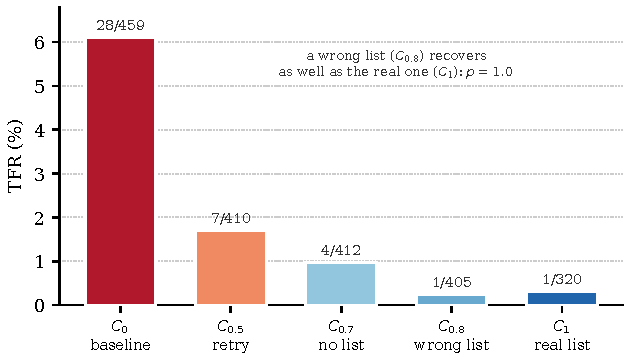
\includegraphics[width=\linewidth]{figures/figC_qwen25_ablation}
\caption{Qwen2.5 ablation ladder. A bare retry ($\mathrm{C}_{0.5}$) only
halves the $6.10\%$ baseline, while the structured \texttt{tool\_not\_found}
envelope cuts it about $20\times$; a \emph{wrong} registry list
($\mathrm{C}_{0.8}$) recovers as well as the real one ($\mathrm{C}_1$;
Fisher $p=1.0$), so recovery is format-driven.}
\label{fig:qwen25-ablation}
\end{figure}

\section{Pre-Registration and Reproducibility}
\label{sec:appendix:prereg}

The pre-registered protocol is locked in git commit \texttt{c391017},
dated before any data was collected. Three deviations from that
protocol are worth naming. Probe $N$ was reduced from $100$ to $15$
per cell to fund breadth across five Anthropic versions and six
Qwen3 sizes. The OpenAI gpt-4.1 and gpt-4o tiers were added to the
vendor scope after the pre-registration (five commercial models,
$0/2{,}117$ pooled C0 calls, all $0\%$ TFR). The gpt-5 generation
(gpt-5, gpt-5-mini, gpt-5-nano, gpt-5.5) has since completed and extends
the commercial null: $0/1{,}311$ pooled, all $0\%$ TFR
($\leq\!0.28\%$). We keep these out of the locked $0/2{,}117$ headline
pool and report them as a confirmatory extension. $\mathrm{C}_{0.7}$
was run at scale on Qwen3-8B only, not on Anthropic. Holm--Bonferroni
correction across the three primary tests (Fisher's exact, Friedman,
TOST): only Fisher's clears $\alpha\!=\!0.05$ at
$p_{\mathrm{Holm}} = 1.0\!\times\!10^{-4}$.

\begin{figure}[tb]
\centering
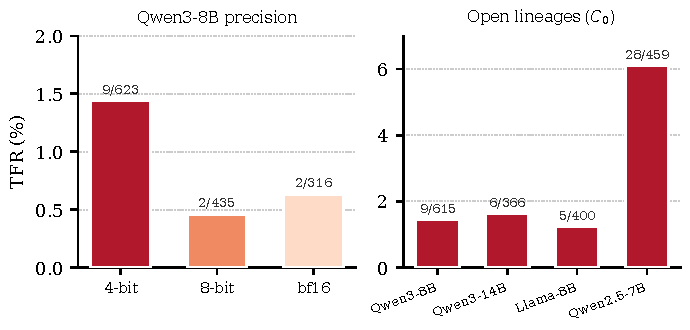
\includegraphics[width=\linewidth]{figures/figD_controls}
\caption{Controls. Left: the precision ladder (Qwen3-8B at
4-bit/8-bit/bf16) shows fabrication persists at full precision, so it is
not a quantization artefact. Right: the $\mathrm{C}_0$ fabrication rate
across open lineages.}
\label{fig:controls}
\end{figure}

The supplementary repository at
\href{https://github.com/Akasxh/tool-fabrication-rate}{github.com/Akasxh/tool-fabrication-rate}
contains the full harness ($153$ unit tests), the JSONL trace logs
that produce every number in the paper, the aggregator and statistical
scripts, the reproducibility manifest with dated model aliases, the
full deviation log, the JSONL trace schema, the headline-number
derivation rule, and a registry-size pilot. Running
\texttt{python scripts/aggregate\_all.py} on the released traces
reproduces every numerical claim. Distractor-injection RNG uses a
SHA-256-derived stable hash, so reproduction does not depend on
\texttt{PYTHONHASHSEED}; MLX 4-bit local inference is not
bitwise-deterministic across runs but per-task tool-call decisions
are stable to within $\pm 1$ token.

\section{Broader Impacts and Responsible Disclosure}
\label{sec:appendix:impacts}
This work is diagnostic and defensive: it measures a failure mode and
ships a training-free mitigation. Every fabrication reported here was
elicited in a typed, offline harness with no real executor and no side
effects. We demonstrate no exploit and trigger no real-world action.
The underlying failure class (agents emitting calls to non-existent
tools) is already documented in prior tool-hallucination
work~\citep{li2023apibank,huang2024metatool}, and the open-weight models
we name are publicly released, so we judge the net effect of releasing a
per-call measurement plus a cheap fix to be defensive rather than
uplifting. The one concrete risk we surface (a \emph{permissive}
executor that fuzzy-matches or auto-registers a fabricated
state-changing call) is mitigated by the executor-side allow-listing
we recommend alongside RVR; RVR reduces the fabrication load reaching
that allow-list rather than replacing it. Code and the per-event
severity labels are released at
\href{https://github.com/Akasxh/tool-fabrication-rate}{github.com/Akasxh/tool-fabrication-rate}
to support reproduction and defensive tooling.
